\documentclass[10pt,a4paper]{article}

\usepackage[T1]{fontenc}
\usepackage[utf8]{inputenc}
\usepackage{lmodern}
\usepackage[margin=20mm,headheight=15pt]{geometry}
\usepackage{microtype}
\usepackage[table]{xcolor}
\usepackage{booktabs}
\usepackage{longtable}
\usepackage{tabularx}
\usepackage{array}
\usepackage{enumitem}
\usepackage{pdflscape}
\usepackage{float}
\usepackage{fancyhdr}
\usepackage{titlesec}
\usepackage{tikz}
\usetikzlibrary{arrows.meta,positioning}
\usepackage{hyperref}

\definecolor{accent}{HTML}{0E7490}
\definecolor{Navy}{HTML}{17324D}
\definecolor{Sky}{HTML}{E8F1FA}
\definecolor{Mint}{HTML}{EAF7F4}
\definecolor{Gray}{HTML}{F3F4F6}

\hypersetup{
  colorlinks=true,
  linkcolor=black,
  citecolor=black,
  urlcolor=accent,
  pdftitle={Google Cloud Analytics Platform: Architecture and Bitcoin Cash Pipeline Evidence},
  pdfauthor={Daniel Bostan}
}
\urlstyle{same}
\sloppy
\setlength{\emergencystretch}{2em}

\pagestyle{fancy}
\fancyhf{}
\fancyhead[L]{\small GCP Analytics Platform \textbullet{} BCH Evidence}
\fancyhead[R]{\small\thepage}
\renewcommand{\headrulewidth}{0.4pt}

\titleformat{\section}{\large\bfseries\color{accent}}{\thesection}{0.6em}{}
\titleformat{\subsection}{\normalsize\bfseries}{\thesubsection}{0.55em}{}
\titlespacing*{\section}{0pt}{11pt}{4pt}
\titlespacing*{\subsection}{0pt}{8pt}{3pt}
\setlist[itemize]{leftmargin=*,itemsep=2pt,topsep=3pt}
\setlist[enumerate]{leftmargin=*,itemsep=2pt,topsep=3pt}
\setlength{\parindent}{0pt}
\setlength{\parskip}{0.45em}
\renewcommand{\arraystretch}{1.15}
\setlength{\tabcolsep}{4pt}

\newcolumntype{Y}{>{\raggedright\arraybackslash}X}
\newcolumntype{L}[1]{>{\raggedright\arraybackslash}p{#1}}
\newcommand{\code}[1]{\nolinkurl{#1}}

\begin{document}

%----------------------------------------------------------------------
\begin{titlepage}
\centering
\vspace*{3cm}
{\Huge\bfseries Google Cloud Analytics Platform\par}
\vspace{0.4cm}
{\Large Architecture Design and Bitcoin Cash Pipeline Evidence\par}
\vspace{1.2cm}
{\large Solution to the Astrafy Data Engineer Take-Home Challenge\par}
\vspace{2.2cm}
{\large Daniel Bostan\par}
\vspace{0.9cm}
{\normalsize daniel.bostan@proton.me\par}
\vspace{0.2cm}
{\normalsize \href{https://github.com/Xocket/astrafy-bch-infra}{github.com/Xocket/astrafy-bch-infra}
\quad
\href{https://github.com/Xocket/astrafy-bch-dbt}{github.com/Xocket/astrafy-bch-dbt}\par}
\vfill
{\normalsize September 2026\par}
\end{titlepage}

\tableofcontents
\clearpage

%----------------------------------------------------------------------
\section{AI-assisted development and engineering method}

This project was built as an AI-assisted pair-programming exercise. This
section records which assistants did what, and which work stayed human.
The rule was the same everywhere: the assistant proposes, the human
decides, and a machine gate verifies.

\subsection{Tools and what each did}

\begin{itemize}
  \item \textbf{Roadmap.} Astra planned the execution: the phase order,
        the risk list (cloud onboarding, balance semantics, CI
        authentication), and the time budget.
  \item \textbf{Decisions.} GPT Sol 5.6 analysed each ambiguity in the
        brief and drafted the decision records in \code{docs/adr/}. I
        selected the interpretation in every case.
  \item \textbf{First code.} GPT Luna 5.6 wrote the first Terraform
        stack and the first dbt models.
  \item \textbf{Remaining code and tests.} DeepSeek V4.1 Flash wrote the
        rest of the models, the eight singular tests, and the generic
        test declarations. I changed assistant mid-project when one
        subscription ran out, and continued with the same gates.
  \item \textbf{Documentation.} GPT Sol 5.6 drafted the report, the
        READMEs, and the evidence documents from the repository files
        and the recorded decisions.
  \item \textbf{Final pass.} GLM 5.3, through the local OpenCode
        harness, shortened this report, condensed the repository
        documentation, and checked that every number matches the
        recorded evidence.
\end{itemize}

\subsection{What stayed human}

\begin{itemize}
  \item \textbf{Interpretation.} The brief leaves ``current balance'',
        ``Coinbase'', and the three-month window open. I chose each
        interpretation and recorded it in a decision record.
  \item \textbf{Verification.} I ran the Terraform applies, the dbt
        build, the tests, and the CI myself. A green result was never
        assumed.
  \item \textbf{Security.} I reviewed the IAM scopes and the Workload
        Identity Federation conditions line by line.
  \item \textbf{This text.} I read and approved every part of it.
\end{itemize}

\subsection{Guardrails}

AI output was treated as a draft. These gates ran on every change:
\code{dbt parse} and \code{dbt compile} offline, the 45 dbt tests against
BigQuery, \code{terraform fmt} and \code{validate} with a plan-only CI
job, pre-commit with a private-key scan, and a byte cap on every BigQuery
job (100 GiB locally, 50 GiB in CI). Every measured number in this
report comes from a run log or a repository file, not from an assistant.

%----------------------------------------------------------------------
\section{Executive decision}

\textbf{Recommendation.} Build the platform on Google Cloud in separate
development and production projects. Capture every source into an
immutable raw layer. Transform the data with dbt Core in BigQuery.
Publish one governed semantic layer for all dashboards. Reuse the same
governed features for model training and model serving. Keep all
infrastructure and transformation code in Git: pull requests carry the
evidence, humans approve each promotion.

\begin{tabularx}{\textwidth}{L{36mm}Y}
\toprule
\textbf{Driver} & \textbf{Architectural answer} \\
\midrule
Six different sources & One ingestion contract per source: change data capture for databases, events where the source publishes them, checkpointed APIs otherwise. \\
Several departments & Conformed entities and one semantic layer. Each department gets its own view of the shared metrics. \\
BI and ML together & Features come from governed intermediate data, never from dashboard tables. \\
Open source where practical & dbt Core, Debezium, Airflow, Feast, OpenLineage. Managed services stay where they remove real operating work. \\
GitOps and DataOps & Git is the source of truth. CI produces evidence; protected branches own promotion. \\
Security and privacy & Separate projects, keyless workload identities, classified data, deletion by design. \\
Cost & Partition, cluster, dry-run, cap, budget. The free tier is a guardrail, not a promise. \\
\bottomrule
\end{tabularx}

\textbf{Non-goals.}
\begin{itemize}
  \item Replace operational systems. The design ingests them; it does not migrate them.
  \item Let BI users query production databases directly.
  \item Treat budget alerts as a spending cap. Google budgets notify; they do not block.\cite{gcBudget}
  \item Promise exactly-once outcomes. The design assumes at-least-once delivery and makes processing idempotent.\cite{gcPubSubExactly}
\end{itemize}

\textbf{Acceptance.} A pilot is accepted when the source-to-raw
reconciliation repeats, freshness and completeness targets pass for a
representative period, contract tests block bad changes, the Terraform
plan shows only reviewed changes, workload identities are keyless and
ref-constrained, and cost and scans stay inside approved limits.

%----------------------------------------------------------------------
\section{Part 1: architecture on Google Cloud}

The customer data comes from PostgreSQL, MySQL, MongoDB, SAP, Salesforce,
and SurveyMonkey. The goal is a platform that serves dashboards for
several departments and feeds models for recommendations and
predictions. Figure~\ref{fig:arch} shows the flow: capture, immutable
raw storage, warehouse layers, and consumers.

\begin{landscape}
\begin{figure}[H]
\centering
\resizebox{0.96\linewidth}{!}{%
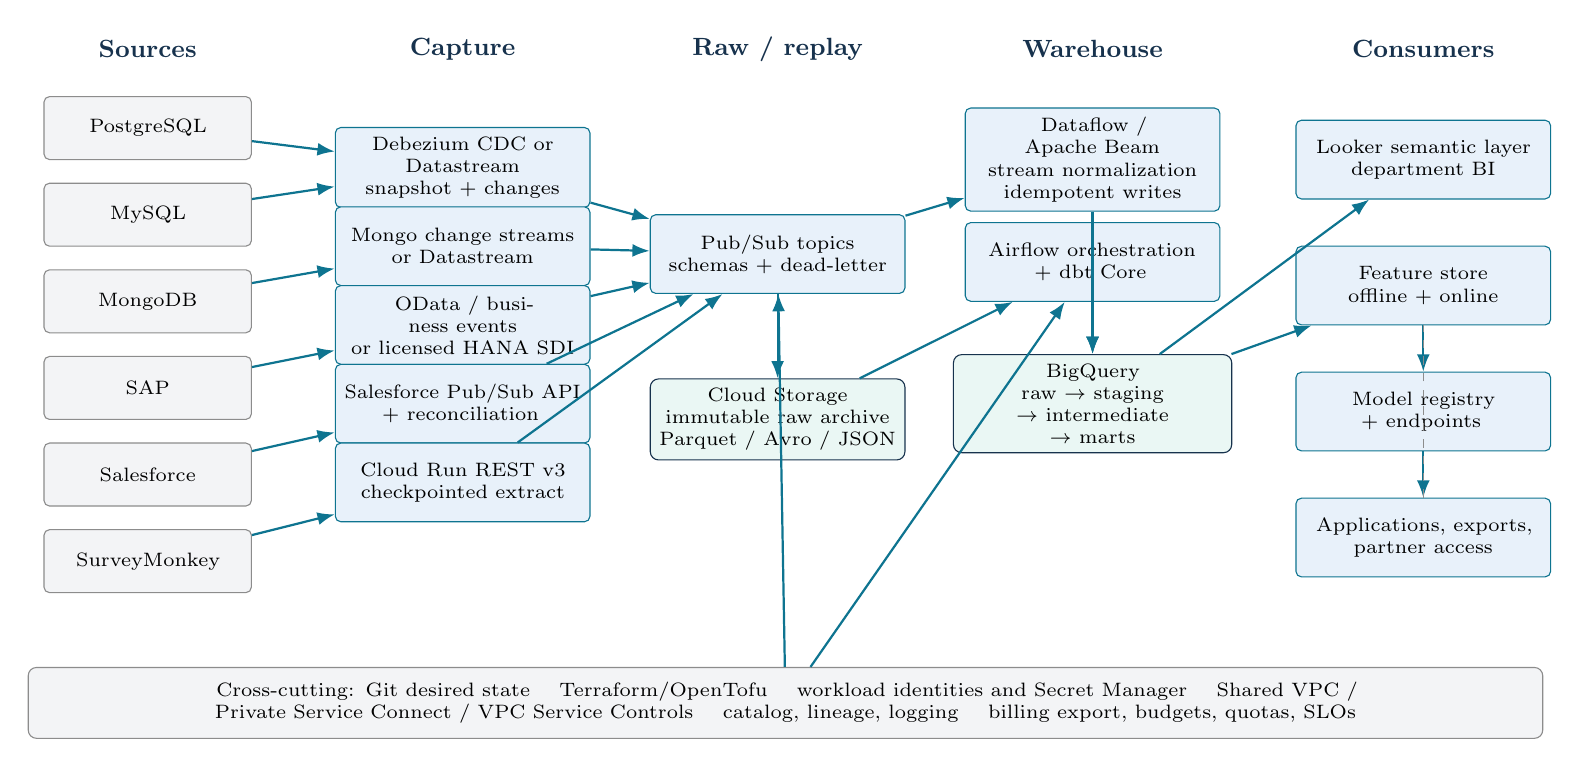
\begin{tikzpicture}[x=1cm,y=1cm,
  srcbox/.style={rectangle,rounded corners=2pt,draw=black!45,fill=Gray,align=center,minimum height=8mm,text width=24mm,font=\scriptsize},
  svcbox/.style={rectangle,rounded corners=2pt,draw=accent,fill=Sky,align=center,minimum height=10mm,text width=30mm,font=\scriptsize},
  datastorebox/.style={rectangle,rounded corners=3pt,draw=Navy,fill=Mint,align=center,minimum height=10mm,text width=30mm,font=\scriptsize},
  flow/.style={-{Latex[length=2.2mm]},line width=0.8pt,draw=accent}]
  \node[font=\small\bfseries\color{Navy}] at (0,8.2) {Sources};
  \node[font=\small\bfseries\color{Navy}] at (4.0,8.2) {Capture};
  \node[font=\small\bfseries\color{Navy}] at (8.0,8.2) {Raw / replay};
  \node[font=\small\bfseries\color{Navy}] at (12.0,8.2) {Warehouse};
  \node[font=\small\bfseries\color{Navy}] at (16.2,8.2) {Consumers};

  \node[srcbox] (pg) at (0,7.2) {PostgreSQL};
  \node[srcbox] (my) at (0,6.1) {MySQL};
  \node[srcbox] (mo) at (0,5.0) {MongoDB};
  \node[srcbox] (sap) at (0,3.9) {SAP};
  \node[srcbox] (sf) at (0,2.8) {Salesforce};
  \node[srcbox] (sm) at (0,1.7) {SurveyMonkey};

  \node[svcbox] (cdc) at (4.0,6.7) {Debezium CDC or\\Datastream\\snapshot + changes};
  \node[svcbox] (docdc) at (4.0,5.7) {Mongo change streams\\or Datastream};
  \node[svcbox] (sapapi) at (4.0,4.7) {OData / business events\\or licensed HANA SDI};
  \node[svcbox] (sfapi) at (4.0,3.7) {Salesforce Pub/Sub API\\+ reconciliation};
  \node[svcbox] (smapi) at (4.0,2.7) {Cloud Run REST v3\\checkpointed extract};

  \node[svcbox] (pubsub) at (8.0,5.6) {Pub/Sub topics\\schemas + dead-letter};
  \node[datastorebox] (gcs) at (8.0,3.5) {Cloud Storage\\immutable raw archive\\Parquet / Avro / JSON};

  \node[svcbox] (beam) at (12.0,6.8) {Dataflow / Apache Beam\\stream normalization\\idempotent writes};
  \node[svcbox] (airflow) at (12.0,5.5) {Airflow orchestration\\+ dbt Core};
  \node[datastorebox,text width=33mm] (bq) at (12.0,3.7) {BigQuery\\raw $\to$ staging\\$\to$ intermediate\\$\to$ marts};

  \node[svcbox] (looker) at (16.2,6.8) {Looker semantic layer\\department BI};
  \node[svcbox] (feat) at (16.2,5.2) {Feature store\\offline + online};
  \node[svcbox] (mlops) at (16.2,3.6) {Model registry\\+ endpoints};
  \node[svcbox] (apps) at (16.2,2.0) {Applications, exports,\\partner access};

  \draw[flow] (pg) -- (cdc);
  \draw[flow] (my) -- (cdc);
  \draw[flow] (mo) -- (docdc);
  \draw[flow] (sap) -- (sapapi);
  \draw[flow] (sf) -- (sfapi);
  \draw[flow] (sm) -- (smapi);
  \draw[flow] (cdc) -- (pubsub);
  \draw[flow] (docdc) -- (pubsub);
  \draw[flow] (sapapi) -- (pubsub);
  \draw[flow] (sfapi) -- (pubsub);
  \draw[flow] (smapi) -- (pubsub);
  \draw[flow] (pubsub) -- (beam);
  \draw[flow] (beam) -- (bq);
  \draw[flow] (pubsub) -- (gcs);
  \draw[flow] (gcs) -- (airflow);
  \draw[flow] (airflow) -- (bq);
  \draw[flow] (bq) -- (looker);
  \draw[flow] (bq) -- (feat);
  \draw[flow] (feat) -- (mlops);
  \draw[flow] (mlops) -- (apps);
  \draw[dashed,black!45] (apps) -- (feat);

  \node[rectangle,rounded corners=3pt,draw=black!45,fill=Gray,align=center,text width=19cm,minimum height=9mm,font=\scriptsize] (cross) at (8.1,-0.1) {Cross-cutting: Git desired state \quad Terraform/OpenTofu \quad workload identities and Secret Manager \quad Shared VPC / Private Service Connect / VPC Service Controls \quad catalog, lineage, logging \quad billing export, budgets, quotas, SLOs};
  \draw[flow] (cross) -- (airflow);
  \draw[flow] (cross) -- (pubsub);
\end{tikzpicture}}
\caption{Proposed platform. Everything above the grey bar is data flow;
everything in it applies to all stages.}
\label{fig:arch}
\end{figure}
\end{landscape}

\subsection{Projects, network, and environments}

\begin{itemize}
  \item \textbf{Folders.} Platform, shared-security, shared-services,
        data-development, data-production. Folder-level IAM and
        organization policies apply at each level.
  \item \textbf{Shared VPC.} One host project owns subnets, NAT, DNS,
        and firewall policy. Data projects attach as service projects.
  \item \textbf{Separate environments.} Development and production are
        separate projects with separate service accounts, secrets, state
        prefixes, and workload identity trust. Production data is not
        readable from development.
  \item \textbf{Private paths.} Private Service Connect and Private
        Google Access for managed endpoints. Identity-Aware Proxy for
        administrative access. Controlled egress only.
  \item \textbf{Service perimeter.} VPC Service Controls around
        BigQuery, storage, and secrets: first in dry-run mode, then
        enforced. The perimeter and IAM are complementary
        controls.\cite{gcVPCSC}
\end{itemize}

\subsection{Component choices}

{\small
\begin{tabularx}{\textwidth}{L{30mm}L{52mm}Y}
\toprule
\textbf{Capability} & \textbf{Selected} & \textbf{Reason} \\
\midrule
Infrastructure as code & Terraform; OpenTofu when policy requires an OSI license & Mature GCP provider. Terraform is BUSL source-available; OpenTofu is MPL-2.0.\cite{tfLicense,openTofuLicense} \\
Database CDC & Debezium; Datastream where managed is preferred & Debezium is portable open source; Datastream covers PostgreSQL, MySQL, MongoDB, Salesforce.\cite{debezium,gcDatastream} \\
Events & Pub/Sub; Kafka when replay, ordering, or scale demand it & Pub/Sub needs no cluster. Idempotent processing is mandatory either way.\cite{gcPubSubExactly} \\
Raw archive & Cloud Storage immutable objects + BigQuery raw & Portable replay and low-cost retention. \\
Transformation & dbt Core & Reviewable SQL with tests, contracts, docs, and lineage metadata.\cite{dbtLicense} \\
Orchestration & Airflow; Composer when managed operations pay & Open source and DAG-as-code.\cite{airflowLicense} \\
Warehouse & BigQuery: raw, staging, intermediate, marts & Partitioned, clustered, governed. \\
BI & Looker semantic layer & Metrics defined once, governed access.\cite{gcLookML,gcLookerAccess} \\
ML & Feature store, model registry, endpoints (Vertex AI); Feast as the portable option & Reuse of governed features for training and serving.\cite{gcFeatureStore,feast} \\
Lineage and metrics & OpenLineage, Marquez, Cloud Logging/Monitoring & Portable lineage events; managed metrics and alerts.\cite{marquezLicense} \\
\bottomrule
\end{tabularx}
}

\subsection{Ingestion per source}

Every connector states its change signal, its checkpoint, and its
delete rule. ``Connected'' is not enough: each connector has a lag target
from source to raw, raw to typed, typed to mart.

{\small
\begin{tabularx}{\textwidth}{L{22mm}L{56mm}Y}
\toprule
\textbf{Source} & \textbf{Capture} & \textbf{Points that matter} \\
\midrule
PostgreSQL & Debezium logical decoding (WAL); Datastream alternative & Snapshot plus LSN checkpoint. Least-privilege replication role. Do not infer a delete from a missing row. \\
MySQL & Debezium row-based binlog; Datastream alternative & GTID or file/position checkpoint. Monitor binlog retention and connector lag. \\
MongoDB & Change streams from a replica set & Resume-token checkpoint. Keep tombstones and schema versions. Do not flatten nested documents without a rule. \\
SAP & OData or business events; HANA SDI where licensed & Keep document ID, version, validity times, and cancellation flags. SAP interfaces are proprietary products.\cite{sapEvents,sapSDI} \\
Salesforce & Pub/Sub API change events plus REST reconciliation & Replay-ID checkpoint. Soft deletes and undeletes need the audit extract.\cite{sfPubSub} \\
SurveyMonkey & Cloud Run scheduled REST v3 extract & Page cursor per survey. Webhooks wake the job; they are not the payload.\cite{smAPI} \\
\bottomrule
\end{tabularx}
}

\textbf{Connector rules.}
\begin{itemize}
  \item Assume at-least-once delivery. Stable keys and deterministic upserts make replay safe.
  \item Schema changes are explicit: a new revision, compatible by default, quarantined when not.
  \item Deletes are data: raw keeps the operation log; staging applies the current-state rule.
  \item Snapshot and stream overlap is safe: deduplicate by source key and version, then reconcile.
  \item Reconcile counts and checksums on a schedule, not only after failures.
\end{itemize}

\subsection{Data layers and standards}

{\small
\begin{tabularx}{\textwidth}{L{24mm}L{58mm}Y}
\toprule
\textbf{Layer} & \textbf{Contents} & \textbf{Rules} \\
\midrule
Raw & Exact source payload, operation, offset, ingest time, schema revision & Append-only. Ingestion identities only. No corrections. \\
Staging & Typed, deduplicated, source-shaped records & Source-level tests. No department logic. \\
Intermediate & Conformed entities, slowly changing dimensions, feature history & Enterprise identity rules. Owner and contract required. \\
Marts & Department fact and dimension tables & Versioned, tested, certified, declared as exposures. \\
Semantic & Metrics, dimensions, joins, access rules & One definition per metric, with owner, grain, and compatibility policy. \\
\bottomrule
\end{tabularx}
}

\textbf{Standards.}
\begin{itemize}
  \item Keep the source ID. Add surrogate keys only in the intermediate and mart layers.
  \item Store UTC timestamps plus the business time zone where the calendar matters.
  \item Store money as decimals with an explicit currency. Never binary floating point for financial facts.
  \item Keep event time, commit time, ingest time, and publication time separate.
  \item Define deletion once for raw, aggregates, features, exports, and backups. A table drop is not a privacy design.
\end{itemize}

%----------------------------------------------------------------------
\section{Delivery: GitOps and data quality}

Git is the desired state for infrastructure, models, semantic
definitions, and features. A merge is not a release. Pull requests carry
the change and its evidence; protected branches own the promotion.

\textbf{Pull-request evidence.} Format, lint, secret, and policy checks;
\code{dbt parse} and compile with unit tests; a Terraform plan with a
policy and cost diff; a sandbox build with model tests, a data diff, and
a scan estimate.

\textbf{Promotion gates.} Infrastructure needs an approved plan and a
post-apply smoke test. A connector needs source-owner approval, a network
path, and a canary offset. A dbt model needs a full build, a consumer
impact check, and a cost check. A semantic change needs owner
certification and a dashboard check. A model needs registry approval and
a canary endpoint. Rollback is part of every plan: revert the release,
pause schedules, replay from the checkpoint, reconcile.

\textbf{Contracts.} A dataset is production-ready when its schema,
grain, owner, quality thresholds, freshness target, compatibility policy,
and deletion rule are written down. dbt contracts enforce the declared
shape before the build; tests check the content after
it.\cite{dbtContracts}

\textbf{Quality.} Tests cover validity, completeness, uniqueness,
consistency, freshness, and accuracy. Blocking tests fail the build.
Non-blocking tests open an incident with the data product owner.

\textbf{Lineage.} Connector runs emit source, offset range, and schema
revision. The dbt manifest maps models to tests, owners, and exposures.
OpenLineage events land in Marquez; a managed catalog is optional
enrichment.\cite{openlineageDBT,dbtExposures}

\textbf{Incidents.} Detect (freshness, reconciliation, contract, or cost
alert). Contain (pause the schedule, quarantine bad messages, keep the
evidence). Correct (fix the code or contract, replay from the last
trusted checkpoint). Reconcile, republish, and add a regression test.

%----------------------------------------------------------------------
\section{BI for departments and ML reuse}

\subsection{BI}

Define each shared metric once in a version-controlled semantic layer.
Departments compose their own views from the shared definitions; none of
them redefines the metric.\cite{gcLookML,gcLookerAccess}

\begin{itemize}
  \item \textbf{Shared foundation:} customer, product, geography,
        calendar, currency, consent. Centrally owned and certified.
  \item \textbf{Domain semantic:} pipeline, orders, finance, survey
        response. The domain owner approves grain and definition.
  \item \textbf{Department experience:} dashboards and scheduled
        delivery under row and field access control. No hidden metric
        logic.
  \item \textbf{Certified extracts} only for tools that cannot query the
        semantic layer. Export a stable contract.
  \item \textbf{Query budgets.} Replace repeated expensive logic with
        governed aggregates.
  \item \textbf{Impact.} Record dashboards as dbt exposures so model
        changes show their consumers.\cite{dbtExposures}
\end{itemize}

\subsection{ML}

Recommendation and prediction models reuse the warehouse. They do not
build private pipelines.

\begin{itemize}
  \item Features come from governed intermediate data, not from
        notebooks or dashboard marts.
  \item A feature definition states entity key, event time, availability
        time, owner, and version.
  \item Training sets use point-in-time joins, so a feature is visible
        only after it existed.\cite{feast}
  \item The same definition and code serve offline training and online
        serving. Parity and freshness are tested.
  \item Datasets, code, parameters, artifacts, and approvals are
        versioned in a model registry.\cite{gcModelRegistry}
  \item Predictions are logged with model version and policy decision,
        with the minimum personal data.
  \item Monitoring covers feature drift, prediction drift, latency,
        segment performance, and feedback quality.\cite{gcModelMonitoring}
  \item Feedback enters training only after label maturity and human
        approval.
\end{itemize}

%----------------------------------------------------------------------
\section{Security, privacy, and reliability}

\subsection{Identity and access}

\begin{itemize}
  \item People log in through the corporate identity provider with MFA.
        Shared accounts are prohibited.
  \item Workloads use attached service accounts. No service-account keys
        in Git, CI variables, or images. Workload Identity Federation
        gives CI short-lived credentials under owner, repository, ref,
        and actor conditions.\cite{gcWIF}
  \item CI gets only the permission the stage needs. Production roles are
        separate from development roles.
  \item Break-glass access is time-bound, approved, logged, and
        reconciled back to Git.
\end{itemize}

\subsection{Secrets and encryption}

External credentials live in Secret Manager with pinned versions and
audited access.\cite{gcSecret} Cloud KMS customer-managed keys protect
high-value datasets and buckets; key administration is separate from
data administration. TLS in transit, mTLS where supported. Logs never
contain tokens, raw payloads, or personal data.

\subsection{Privacy}

Classify fields (public, internal, confidential, restricted). Minimize
and tokenize identifiers before reuse. Define deletion across raw,
aggregates, features, exports, and backups, and test the deletion path
before production.

\subsection{Reliability and recovery}

{\small
\begin{tabularx}{\textwidth}{L{34mm}L{20mm}L{20mm}Y}
\toprule
\textbf{Tier} & \textbf{RPO} & \textbf{RTO} & \textbf{Recovery method} \\
\midrule
Tier 0: payments, live recommendations & 15 min & 4 h & Warm regional capacity; replay from raw. \\
Tier 1: department dashboards & 1 h & 8 h & Restore objects, redeploy, rebuild curated layers. \\
Tier 2: exploration, batch history & 24 h & 2 days & Rerun from versioned raw. \\
\bottomrule
\end{tabularx}
}

These targets are proposals; the owners approve them. The design keeps
immutable raw data and connector checkpoints, and tests replay. Terraform
state lives in a separate versioned backend. IAM, secret references, and
policies are recreated from Git after a regional loss. Managed BigQuery
disaster recovery is an Enterprise Plus option (about 15-minute
replication, five-minute recovery after initiation).\cite{gcBQDR}
Rehearse the critical paths quarterly.

%----------------------------------------------------------------------
\section{Cost and licensing}

\subsection{Cost control}

Google gives each billing account 1 TiB of free on-demand query processing
and 10 GiB of free storage per month.\cite{gcBQPricing} This is an
allowance for those two services, not a promise about the platform:
orchestration, BI, egress, logging, and online ML bill separately.

{\small
\begin{tabularx}{\textwidth}{L{34mm}Y}
\toprule
\textbf{Control} & \textbf{Implementation} \\
\midrule
Query design & Partition by date, cluster by common filters, select only the needed columns.\cite{gcBQPartitions} \\
Dry-run gate & Estimate every material build; fail above a set threshold. \\
Per-job cap & Maximum bytes billed per query: 100 GiB locally and 50 GiB in CI, as used and measured in this project.\cite{gcBQCosts,gcBQQuotas} \\
Monthly envelope & Alert before 0.8 TiB processed; tune from measured billing data. \\
Budgets & 50/90/100\% alerts. Budgets notify; they do not stop spending.\cite{gcBudget} \\
Attribution & Label jobs by project, team, and data product. Export billing data to BigQuery. \\
Cadence & Weekly top-spend review; monthly unit cost and forecast. \\
\bottomrule
\end{tabularx}
}

Buy reservations only after four weeks of measured use. Managed
disaster recovery, BI, and online feature stores can cost more than the
warehouse itself; cost them as first-class services.

\subsection{Licensing}

Three terms, used consistently. \emph{Open source}: an OSI-approved
license. \emph{Source-available}: the source is published, the rights
are limited. \emph{Managed}: the vendor runs the service under
commercial terms; an open-source SDK does not make the service open.

{\small
\begin{tabularx}{\textwidth}{L{44mm}L{38mm}Y}
\toprule
\textbf{Component} & \textbf{License} & \textbf{Class and note} \\
\midrule
PostgreSQL & PostgreSQL License & Open source.\cite{postgresLicense} \\
MySQL Community & GPLv2 plus exceptions & Open source; enterprise editions are commercial.\cite{mysqlLicense} \\
MongoDB Community & SSPL & Source-available, not OSI. Atlas is managed.\cite{mongoSSPL} \\
Debezium & Apache-2.0 & Open source.\cite{debeziumLicense} \\
Apache Kafka & Apache-2.0 & Open source; self-managed clusters are operating work.\cite{kafkaLicense} \\
Apache Airflow & Apache-2.0 & Open source; Composer is managed.\cite{airflowLicense} \\
dbt Core & Apache-2.0 & Open source; hosted dbt services are managed.\cite{dbtLicense} \\
Terraform & BUSL 1.1 & Source-available. OpenTofu (MPL-2.0) is the open policy option.\cite{tfLicense,openTofuLicense} \\
Feast & Apache-2.0 & Open source; online stores are operating work.\cite{feastLicense} \\
OpenLineage / Marquez & Apache-2.0 & Open source.\cite{marquezLicense} \\
Grafana OSS & AGPL-3.0 & Open source; Grafana Cloud is managed.\cite{grafanaLicense} \\
BigQuery, Pub/Sub, Dataflow, Datastream, Looker, Vertex AI & Commercial & Managed services. \\
SAP, Salesforce, SurveyMonkey interfaces & Commercial & Proprietary APIs and products. \\
\bottomrule
\end{tabularx}
}

%----------------------------------------------------------------------
\section{Alternatives, risks, and rollout}

{\small
\begin{tabularx}{\textwidth}{L{26mm}L{44mm}Y}
\toprule
\textbf{Area} & \textbf{Selected} & \textbf{Switch when} \\
\midrule
Warehouse & BigQuery & Portability or concurrency economics dominate. \\
CDC & Debezium + Datastream option & A source is immutable or low-change: batch is enough. \\
Events & Pub/Sub & Sustained throughput, long replay, or many consumers justify Kafka. \\
Streaming & Dataflow / Beam & The team already runs Spark on GKE. \\
Orchestration & Airflow & Managed operations pay more than flexibility. \\
BI & Looker & Departments demand Power BI or Tableau; keep the certified contracts either way. \\
Feature store & Vertex AI & Portability outweighs managed serving (Feast). \\
IaC & Terraform & Policy requires an OSI license (OpenTofu). \\
\bottomrule
\end{tabularx}
}

\textbf{Main risks and responses.}
\begin{itemize}
  \item Source volumes and API rights are unknown until discovery. Measure before committing to Kafka, Dataflow, or reservations.
  \item SAP and SurveyMonkey depend on licensed interfaces and plan limits. Confirm in the workshop; keep the incremental fallback.
  \item Metric duplication: without a governed semantic layer, departments silently redefine revenue.
  \item Feature leakage: without availability timestamps and point-in-time joins, models validate well and fail live.
  \item The free tier is finite. This project measured about 958 GiB for one full pipeline run (Section~\ref{sec:cost}). Caps and budgets control repeats.
\end{itemize}

\textbf{Rollout.} Discover and contract first: source inventory, owners,
classifications, volumes, service targets, and a cost baseline (weeks
0--3). Build the foundation: projects, network, identities, state, and
observability (3--7). Pilot one database and one application source end
to end (6--11). Expand to the remaining sources and full operations
(10--16). Department BI (15--21), then the first bounded ML use case
(20--27). Run old and new outputs in parallel for one business cycle.
Reconcile totals, grain, and definitions, not just numbers. Migrate one
department at a time. Keep rollback until sign-off.

%----------------------------------------------------------------------
\clearpage
\section{Part 2: the Bitcoin Cash pipeline, as built}
\label{sec:part2}

Part 1 is a design. Part 2 is implemented and verified. Everything in
this section comes from the two public repositories and from recorded
runs.\cite{repoInfra,repoDBT} The evidence date is 24 September 2026.

\subsection{Infrastructure (Terraform)}

\begin{itemize}
  \item \textbf{Bootstrap stack.} A dedicated state project, one private
        versioned GCS bucket, a read-only plan service account, and an
        EUR 2 alert budget at 50/90/100\%. Bootstrap state is local and
        gitignored.
  \item \textbf{Primary stack.} Dev project
        \code{astrafy-thc-006-xocket} (number 132073509225), US
        \code{staging}/\code{marts} datasets, required APIs, the dbt
        service account, IAM, and the workload identity pool and
        provider. State prefix \code{astrafy-bch-analytics/dev} in the
        bootstrap bucket; prod uses a separate prefix and stays
        un-applied.
  \item \textbf{dbt identity.} Project-level
        \code{roles/bigquery.jobUser}, a custom role with only
        \code{datasets.create/get}, and \code{dataEditor} on the two
        owned datasets. It is not dataEditor on the public dataset.
  \item \textbf{Source view.} The organization cannot change the public
        dataset IAM, so Terraform creates
        \code{staging.bch_transactions_source}: a view over
        \code{bigquery-public-data.crypto_bitcoin_cash.transactions}
        that renames the reserved column \code{hash} to
        \code{transaction_hash}. The view runs with its creator's
        access.
  \item \textbf{No static key.} There is no service-account-key
        resource, no credential variable, and no JSON fallback.
  \item \textbf{CI.} Format and validate run always. An authenticated
        read-only plan runs on main with workload identity. No workflow
        can apply.
\end{itemize}

\subsection{dbt models}

\begin{verbatim}
bch_transactions_source (Terraform view over
bigquery-public-data.crypto_bitcoin_cash.transactions)
                              |
                    stg_analysis_window
                              |
                    stg_transactions (table)
                       /              \
stg_protocol_coinbase_addresses   stg_address_ledger
                       \              /
                        address_balances
\end{verbatim}

\begin{itemize}
  \item \code{stg_analysis_window} captures
        \code{max(block_timestamp)} once and derives the inclusive start
        at midnight exactly three calendar months earlier. The capture
        timestamp is audit data; it does not define the window.
  \item \code{stg_transactions} is a table partitioned by month and
        clustered by hash. Hash deduplication is deterministic. The
        nested arrays keep only index, addresses, and value.
  \item \code{stg_protocol_coinbase_addresses} collects the non-empty
        output addresses of transactions with
        \code{is_coinbase = true} in the same window.
  \item \code{stg_address_ledger} turns each address element into its
        own row: trims whitespace, filters null, empty, and sentinel
        addresses, keeps the source case, makes inputs negative and
        outputs positive, and drops the excluded addresses.
  \item \code{address_balances} groups the ledger by address, keeps
        exact satoshis, and exposes
        \code{balance_bch = balance_satoshis / 100000000}.
\end{itemize}

Every generated table carries workload labels and a seven-day
expiration, so abandoned tables cannot bill storage indefinitely.

\subsection{Live results}
\label{sec:cost}

The public source ends on 2024-05-13, so the window is source-relative,
not wall-clock. Measured on 24 September 2026:

{\small
\begin{tabularx}{\textwidth}{L{56mm}Y}
\toprule
\textbf{Measurement} & \textbf{Value} \\
\midrule
Window & 2024-02-13T00:00:00+00:00 to 2024-05-13T23:57:05+00:00, inclusive \\
Staged transactions & 6,495,376 \\
Protocol-coinbase transactions in window & 13,230 \\
Excluded protocol-coinbase addresses & 4,544 \\
Ledger rows & 35,686,444 \\
Mart addresses & 5,774,930 \\
Net movement across all mart addresses & 6.47 trillion satoshis \\
Addresses with a negative balance & about 1.06 million (valid; see semantics) \\
Table storage & 12.54 GiB logical; seven-day expiration; labels verified \\
Query scan, full run & about 958 GiB; \code{stg_transactions} alone: 945.6 GiB \\
Latest-timestamp query estimate & 2.91 GiB (3,127,792,896 bytes) \\
Three-month profile estimate & 6.19 GiB (6,646,559,904 bytes) \\
Tests & 45 passed, 0 failed, 0 warned \\
\bottomrule
\end{tabularx}
}

\subsection{Semantics}

\begin{itemize}
  \item \textbf{Balance} is the three-month net movement: outputs minus
        inputs inside the captured window. It is not a lifetime balance.
        A negative value is valid: the funding can be older than the
        window.
  \item \textbf{Coinbase} is the protocol coinbase flag, not the
        exchange. No authoritative exchange-address list exists in the
        source; the interpretation is deterministic and recorded
        (ADR 0003).
  \item \textbf{Addresses} are trimmed, not lower-cased. Base58 and
        Bech32 case is not safely interchangeable.
  \item \textbf{Multisig} outputs credit each listed address. This is
        attribution, not beneficial ownership.
  \item \textbf{Fees} stay on the transaction and are checked per
        transaction; they are never assigned to an address.
\end{itemize}

\subsection{Tests}

45 tests ran against the live tables: 37 generic (not-null, unique,
accepted values, window bounds) and 8 singular assertions:

\begin{itemize}
  \item \code{assert_captured_window} --- the window is exactly three
        calendar months, inclusive, and the staged maximum equals the
        captured maximum.
  \item \code{assert_stg_transactions_within_window} --- no staged
        row outside the window or its partition bounds.
  \item \code{assert_transaction_accounting} --- for complete
        non-coinbase rows, input = output + fee.
  \item \code{assert_protocol_coinbase_addresses} --- the exclusion
        set equals the non-empty coinbase output addresses in the window.
  \item \code{assert_protocol_coinbase_exclusion} --- excluded
        addresses appear in neither the ledger nor the mart.
  \item \code{assert_no_sentinel_addresses} --- null, empty, and
        textual-null sentinels are absent.
  \item \code{assert_ledger_entry_uniqueness} --- no duplicate ledger
        rows.
  \item \code{assert_balance_equation} --- signed balance equals
        outputs minus inputs, and the BCH conversion is exact.
\end{itemize}

All 45 passed in the local full run and in CI (pull request and main).

\subsection{CI and authentication}

\begin{itemize}
  \item Triggers: pull request opened, synchronized, or reopened, and
        push to \code{main}. Superseded runs cancel.
  \item A credential-free job runs \code{dbt parse
        --no-partial-parse} on every trigger.
  \item The authenticated job uses workload identity federation to the
        Terraform-provisioned service account. Both jobs passed in run
        \href{https://github.com/Xocket/astrafy-bch-dbt/actions/runs/36054350409}{36054350409}.
  \item Steps: \code{dbt compile --no-introspect}, a cost-capped
        \code{dbt run --select address_balances}, \code{dbt test}, and
        \code{dbt docs generate}. Artifacts upload for 14 days.
  \item The full five-model refresh is manual: the measured 945.6 GiB
        source scan is close to the 1 TiB monthly allowance.
  \item The workload identity CEL conditions pin owner, repository,
        ref, event, and actor. Infrastructure CI is main-only; dbt
        development trust also accepts owner-initiated pull requests;
        production accepts dbt main only. Bindings are exact principal
        sets.
  \item The infrastructure plan job authenticated with workload
        identity and found no drift:
        \href{https://github.com/Xocket/astrafy-bch-infra/actions/runs/36054422871}{run
        36054422871}.
\end{itemize}

\subsection{Honest status}

{\small
\begin{tabularx}{\textwidth}{L{44mm}L{62mm}L{22mm}}
\toprule
\textbf{Claim} & \textbf{Evidence} & \textbf{Status} \\
\midrule
Datasets, service account, WIF exist & Terraform outputs; inspection & Verified \\
Bootstrap and primary stacks applied & Applied; outputs recorded & Verified \\
Five dbt models, 45 tests, docs & Local full run; CI run 36054350409 & Verified \\
Credential-free parse & Same CI run 36054350409 & Verified \\
Public repositories & Both GitHub URLs & Verified \\
Full workload inside the free tier & One full run about 958 GiB; caps and budget in place & Guardrail, not a guarantee \\
Billing reconciliation & BigQuery billing export not yet reviewed & Open \\
Human review and submission & Pending recipient name & Open \\
\bottomrule
\end{tabularx}
}

Two gates remain human: reconcile the BigQuery billing export for the
measured run, and review this PDF, attach it, and send the reply email.

%----------------------------------------------------------------------
\clearpage
\phantomsection
\section*{References}
\addcontentsline{toc}{section}{References}
\footnotesize
\sloppy
All web sources were accessed on 24 September 2026. Vendor documentation
and prices can change; verify them again at procurement time.

\begin{thebibliography}{99}

\bibitem{gcDatastream}
Google Cloud, \emph{Datastream overview}.
\url{https://docs.cloud.google.com/datastream/docs/overview}

\bibitem{gcBQPricing}
Google Cloud, \emph{BigQuery pricing}.
\url{https://cloud.google.com/bigquery/pricing}

\bibitem{gcBQPartitions}
Google Cloud, \emph{Introduction to partitioned tables}.
\url{https://docs.cloud.google.com/bigquery/docs/partitioned-tables}

\bibitem{gcBQCosts}
Google Cloud, \emph{Estimate and control costs}.
\url{https://docs.cloud.google.com/bigquery/docs/best-practices-costs}

\bibitem{gcBQQuotas}
Google Cloud, \emph{Create custom query quotas}.
\url{https://docs.cloud.google.com/bigquery/docs/custom-quotas}

\bibitem{gcPubSubExactly}
Google Cloud, \emph{Exactly-once delivery}.
\url{https://docs.cloud.google.com/pubsub/docs/exactly-once-delivery}

\bibitem{gcWIF}
Google Cloud, \emph{Workload Identity Federation}.
\url{https://docs.cloud.google.com/iam/docs/workload-identity-federation}

\bibitem{gcVPCSC}
Google Cloud, \emph{Overview of VPC Service Controls}.
\url{https://docs.cloud.google.com/vpc-service-controls/docs/overview}

\bibitem{gcSecret}
Google Cloud, \emph{Secret Manager best practices}.
\url{https://docs.cloud.google.com/secret-manager/docs/best-practices}

\bibitem{gcBudget}
Google Cloud, \emph{Create, edit, or delete budgets and budget alerts}.
\url{https://docs.cloud.google.com/billing/docs/how-to/budgets}

\bibitem{gcBQDR}
Google Cloud, \emph{Managed disaster recovery}.
\url{https://docs.cloud.google.com/bigquery/docs/managed-disaster-recovery}

\bibitem{gcLookML}
Google Cloud, \emph{Introduction to LookML}.
\url{https://docs.cloud.google.com/looker/docs/what-is-lookml}

\bibitem{gcLookerAccess}
Google Cloud, \emph{Looker access control and permission management}.
\url{https://docs.cloud.google.com/looker/docs/access-control-and-permission-management}

\bibitem{gcFeatureStore}
Google Cloud, \emph{Feature Store overview}.
\url{https://docs.cloud.google.com/gemini-enterprise-agent-platform/machine-learning/featurestore/latest/overview}

\bibitem{gcModelRegistry}
Google Cloud, \emph{Introduction to Model Registry}.
\url{https://docs.cloud.google.com/vertex-ai/docs/model-registry/introduction}

\bibitem{gcModelMonitoring}
Google Cloud, \emph{Introduction to Model Monitoring}.
\url{https://docs.cloud.google.com/vertex-ai/docs/model-monitoring/overview}

\bibitem{dbtContracts}
dbt Labs, \emph{Model contracts}.
\url{https://docs.getdbt.com/docs/mesh/govern/model-contracts}

\bibitem{dbtExposures}
dbt Labs, \emph{Add exposures to your DAG}.
\url{https://docs.getdbt.com/docs/build/exposures}

\bibitem{debezium}
Debezium, \emph{Source connectors}.
\url{https://debezium.io/documentation/reference/stable/connectors/index.html}

\bibitem{sfPubSub}
Salesforce Developers, \emph{Subscribe with Pub/Sub API}.
\url{https://developer.salesforce.com/docs/platform/change-data-capture/guide/cdc-subscribe-pubsub-api.html}

\bibitem{smAPI}
SurveyMonkey, \emph{SurveyMonkey API v3 documentation}.
\url{https://api.surveymonkey.com/v3/docs}

\bibitem{sapEvents}
SAP Help Portal, \emph{Events on SAP Business Accelerator Hub}.
\url{https://help.sap.com/docs/SAP_S4HANA_CLOUD/0f69f8fb28ac4bf48d2b57b9637e81fa/8cbf952e55364254be2da77aa1342aa5.html}

\bibitem{sapSDI}
SAP Help Portal, \emph{SAP HANA Smart Data Integration overview}.
\url{https://help.sap.com/docs/HANA_SMART_DATA_INTEGRATION/bf2f0282053648f8a1ef873e65ded81a/323ff4c3c12040bab8f1222a901dd95d.html}

\bibitem{openlineageDBT}
OpenLineage, \emph{dbt integration}.
\url{https://openlineage.io/docs/integrations/dbt/}

\bibitem{feast}
Feast, \emph{Introduction: open-source offline/online feature store}.
\url{https://docs.feast.dev/}

\bibitem{tfLicense}
HashiCorp, \emph{Terraform LICENSE} (BUSL 1.1 for current releases).
\url{https://raw.githubusercontent.com/hashicorp/terraform/main/LICENSE}

\bibitem{openTofuLicense}
OpenTofu, \emph{LICENSE} (MPL-2.0).
\url{https://raw.githubusercontent.com/opentofu/opentofu/main/LICENSE}

\bibitem{postgresLicense}
PostgreSQL Global Development Group, \emph{PostgreSQL License}.
\url{https://www.postgresql.org/about/licence/}

\bibitem{mysqlLicense}
Oracle MySQL, \emph{MySQL 8.4 Licensing Information} (Community GPLv2 plus exceptions).
\url{https://raw.githubusercontent.com/mysql/mysql-server/8.4/LICENSE}

\bibitem{mongoSSPL}
MongoDB, \emph{Server Side Public License}.
\url{https://www.mongodb.com/legal/licensing/server-side-public-license}

\bibitem{debeziumLicense}
Debezium, \emph{LICENSE} (Apache License 2.0).
\url{https://raw.githubusercontent.com/debezium/debezium/main/LICENSE.txt}

\bibitem{kafkaLicense}
Apache Kafka, \emph{LICENSE} (Apache License 2.0).
\url{https://raw.githubusercontent.com/apache/kafka/trunk/LICENSE}

\bibitem{airflowLicense}
Apache Airflow, \emph{LICENSE} (Apache License 2.0).
\url{https://raw.githubusercontent.com/apache/airflow/main/LICENSE}

\bibitem{dbtLicense}
dbt Core, \emph{LICENSE} (Apache License 2.0).
\url{https://raw.githubusercontent.com/dbt-labs/dbt-core/main/LICENSE}

\bibitem{feastLicense}
Feast, \emph{LICENSE} (Apache License 2.0).
\url{https://raw.githubusercontent.com/feast-dev/feast/master/LICENSE}

\bibitem{marquezLicense}
Marquez, \emph{LICENSE} (Apache License 2.0).
\url{https://raw.githubusercontent.com/MarquezProject/marquez/main/LICENSE}

\bibitem{grafanaLicense}
Grafana, \emph{LICENSE} (AGPL-3.0 for Grafana OSS).
\url{https://raw.githubusercontent.com/grafana/grafana/main/LICENSE}

\bibitem{repoInfra}
Infrastructure repository: \url{https://github.com/Xocket/astrafy-bch-infra}

\bibitem{repoDBT}
dbt and CI repository: \url{https://github.com/Xocket/astrafy-bch-dbt}

\end{thebibliography}
\normalsize

\end{document}
